\chapter{Réalisation d'un mapping de la maquette sur différente positions}
\label{annexe:MapAutre}
Cette annexe vient présenter les autres mesures dédié au mapping de la plaque.

\begin{figure}[H]
    \centering
    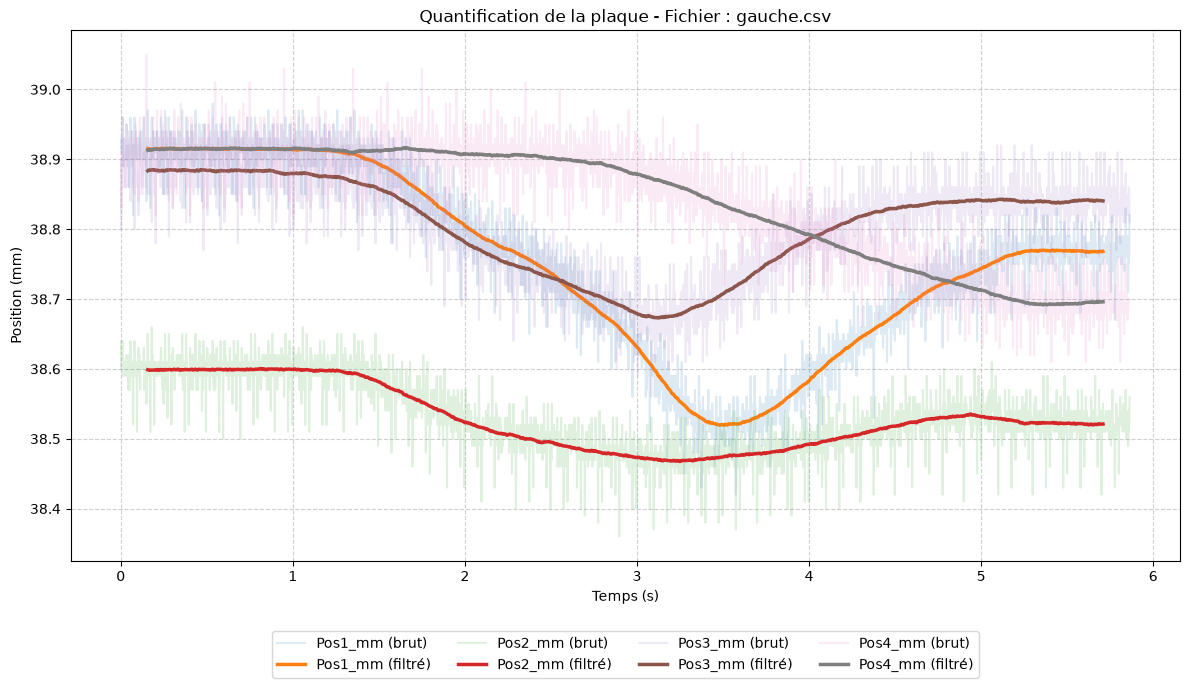
\includegraphics[width=1\linewidth]{assets/appendix/11-Mapping/gauche.png}
    \caption{Mapping de la plaque avec les inducteurs à gauche}
\end{figure}

\begin{figure}[H]
    \centering
    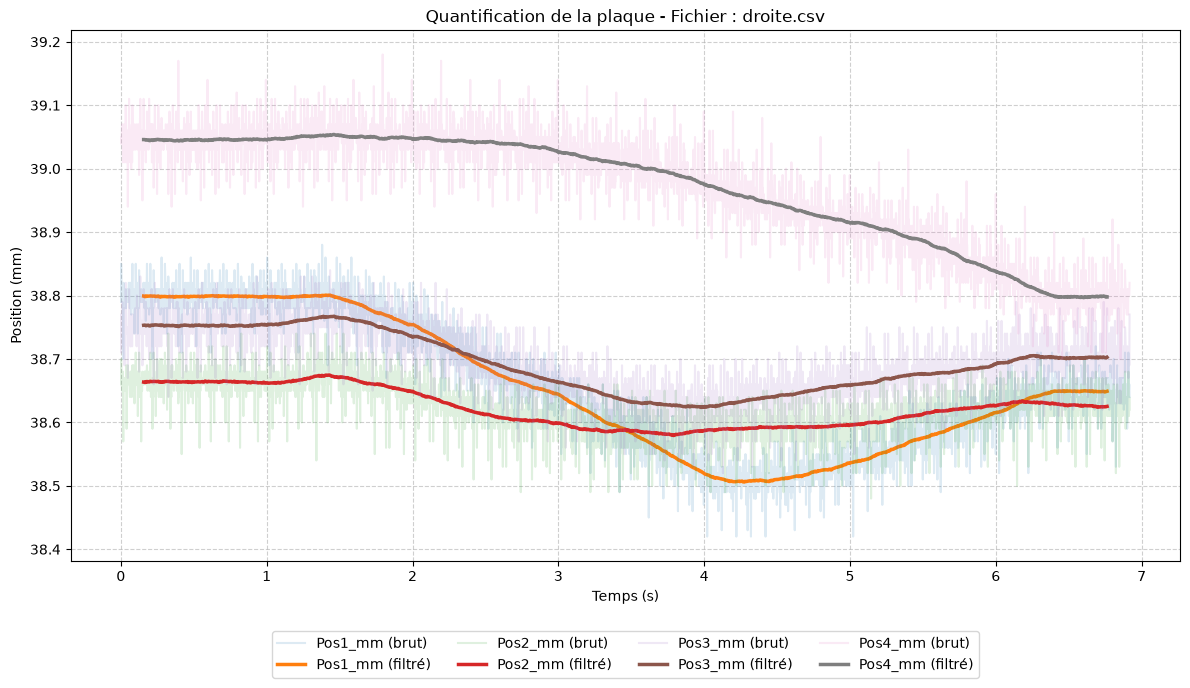
\includegraphics[width=1\linewidth]{assets/appendix/11-Mapping/droite.png}
    \caption{Mapping de la plaque avec les inducteurs à doite}
\end{figure}

\begin{figure}[H]
    \centering
    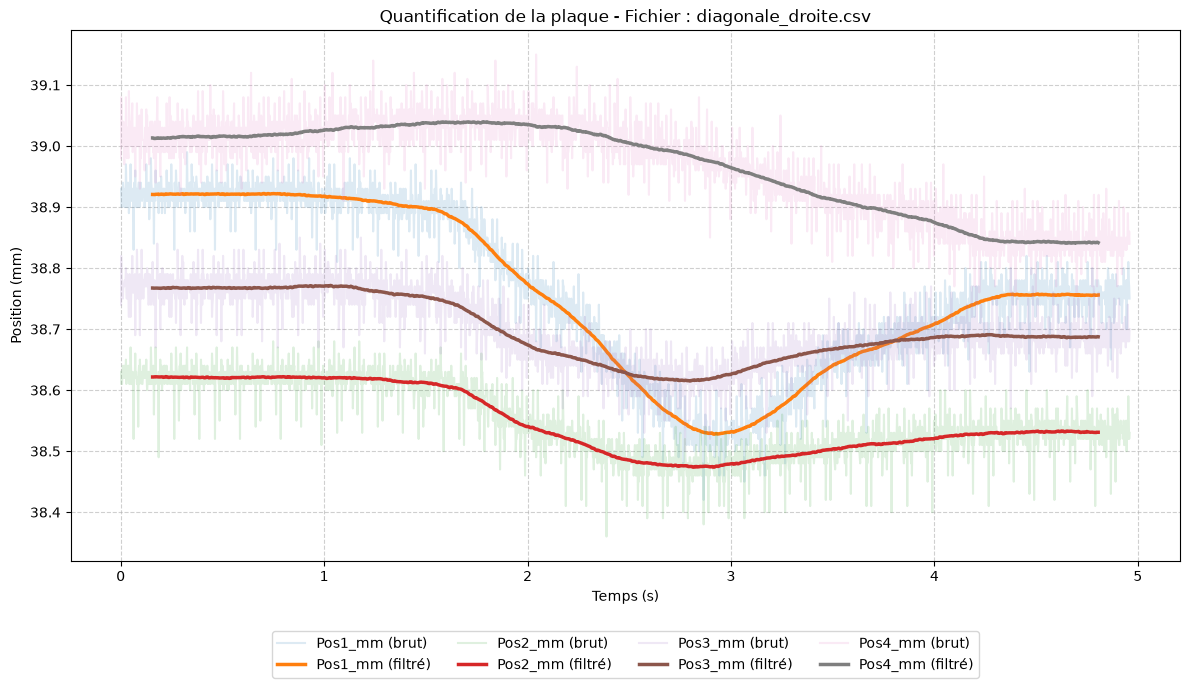
\includegraphics[width=1\linewidth]{assets/appendix/11-Mapping/diagonale_droite.png}
    \caption{Mapping de la plaque avec les inducteurs en diagonale vers la droite}
\end{figure}

\begin{figure}[H]
    \centering
    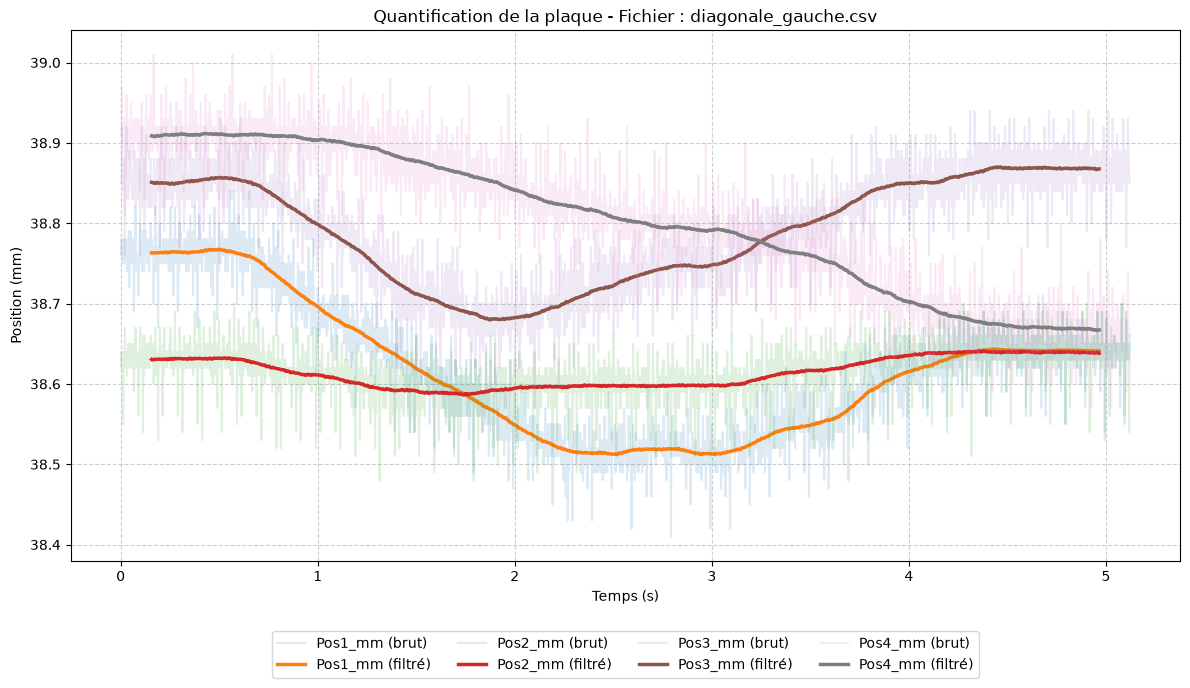
\includegraphics[width=1\linewidth]{assets/appendix/11-Mapping/diagonale_gauche.png}
    \caption{Mapping de la plaque avec les inducteurs en diagonale vers la gauche}
\end{figure}